\section{Κύρια Στοιχεία της Εφαρμογής}
Ακριβώς κάτω από τον χάρτη και την πλαϊνή στήλη βρίσκονται τα κύρια στοιχεία της εφαρμογής. Χωρίζονται σε 5 κατηγορίες "Ταινίες", "Συντελεστές", "Εταιρίες Παραγωγής", "Χώρες Παραγωγής" και "Είδη Ταινιών" όπως φαίνεται στην εικόνα \ref{demo:insights}. 

\begin{figure}[H]
  \centering
  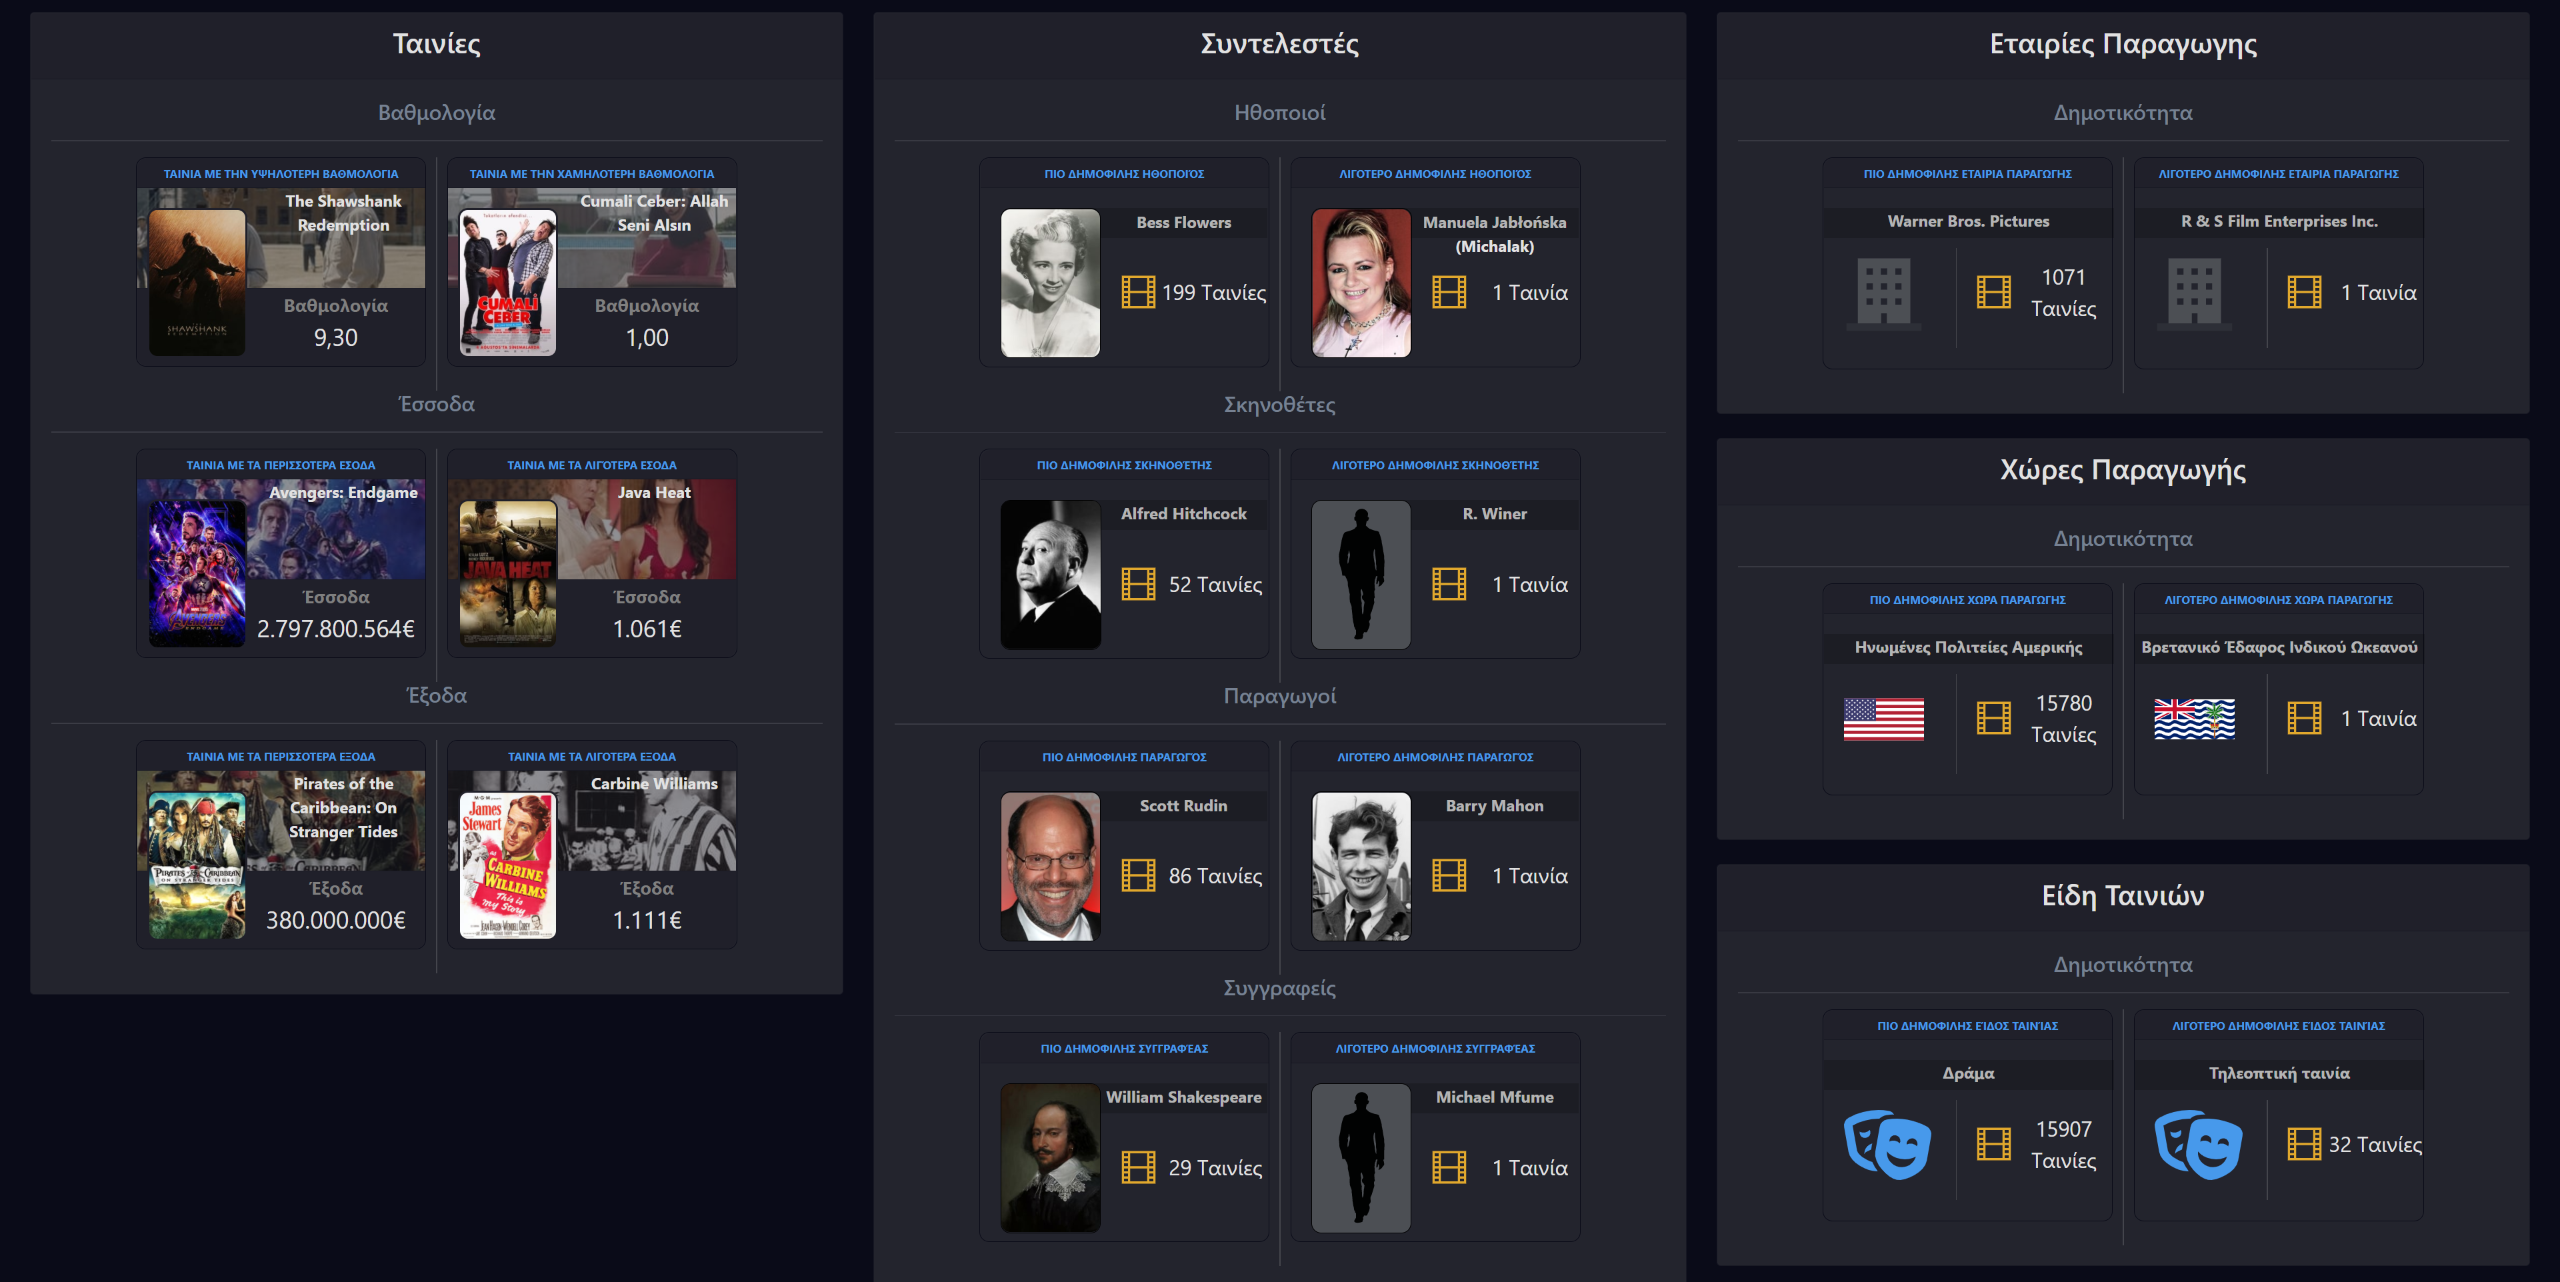
\includegraphics[width=145mm]{Chapters/6 - Manual/Images/main_page_insights.png}
  \caption{Κύρια Στοιχεία της εφαρμογής}
  \label{demo:insights}
\end{figure}

Στην κατηγορία των ταινιών προσφέρονται ταινίες με την μεγαλύτερη και μικρότερη βαθμολογία, και ταινίες με τα περισσότερα και λιγότερα έσοδα και έξοδα. Καθώς ο στόχος της εφαρμογής δεν είναι η προβολή αναλυτικών στοιχείων μιας ταινίας, όταν πατάει ο χρήστης πάνω σε μια από τις κάρτες που εμφανίζονται ανοίγει ένα παραθυράκι προσφέροντας κάποια πολύ βασικά δεδομένα όπως τα έσοδα, έξοδα, η βαθμολογία και ο χρόνος που διαρκεί αυτή η ταινία, και σε περίπτωση που ο χρήστης θέλει να δει παραπάνω στοιχεία για αυτήν την ταινία του δίνεται η δυνατότητα από αυτό το παράθυρο να δει τα στοιχεία που θέλει είτε στην υπηρεσία Internet Movie DataBase (IMDB) είτε στην υπηρεσία The Movie Database (TMDb) όπως φαίνεται στην εικόνα \ref{demo:movie:modal}.

\begin{figure}[H]
  \centering
  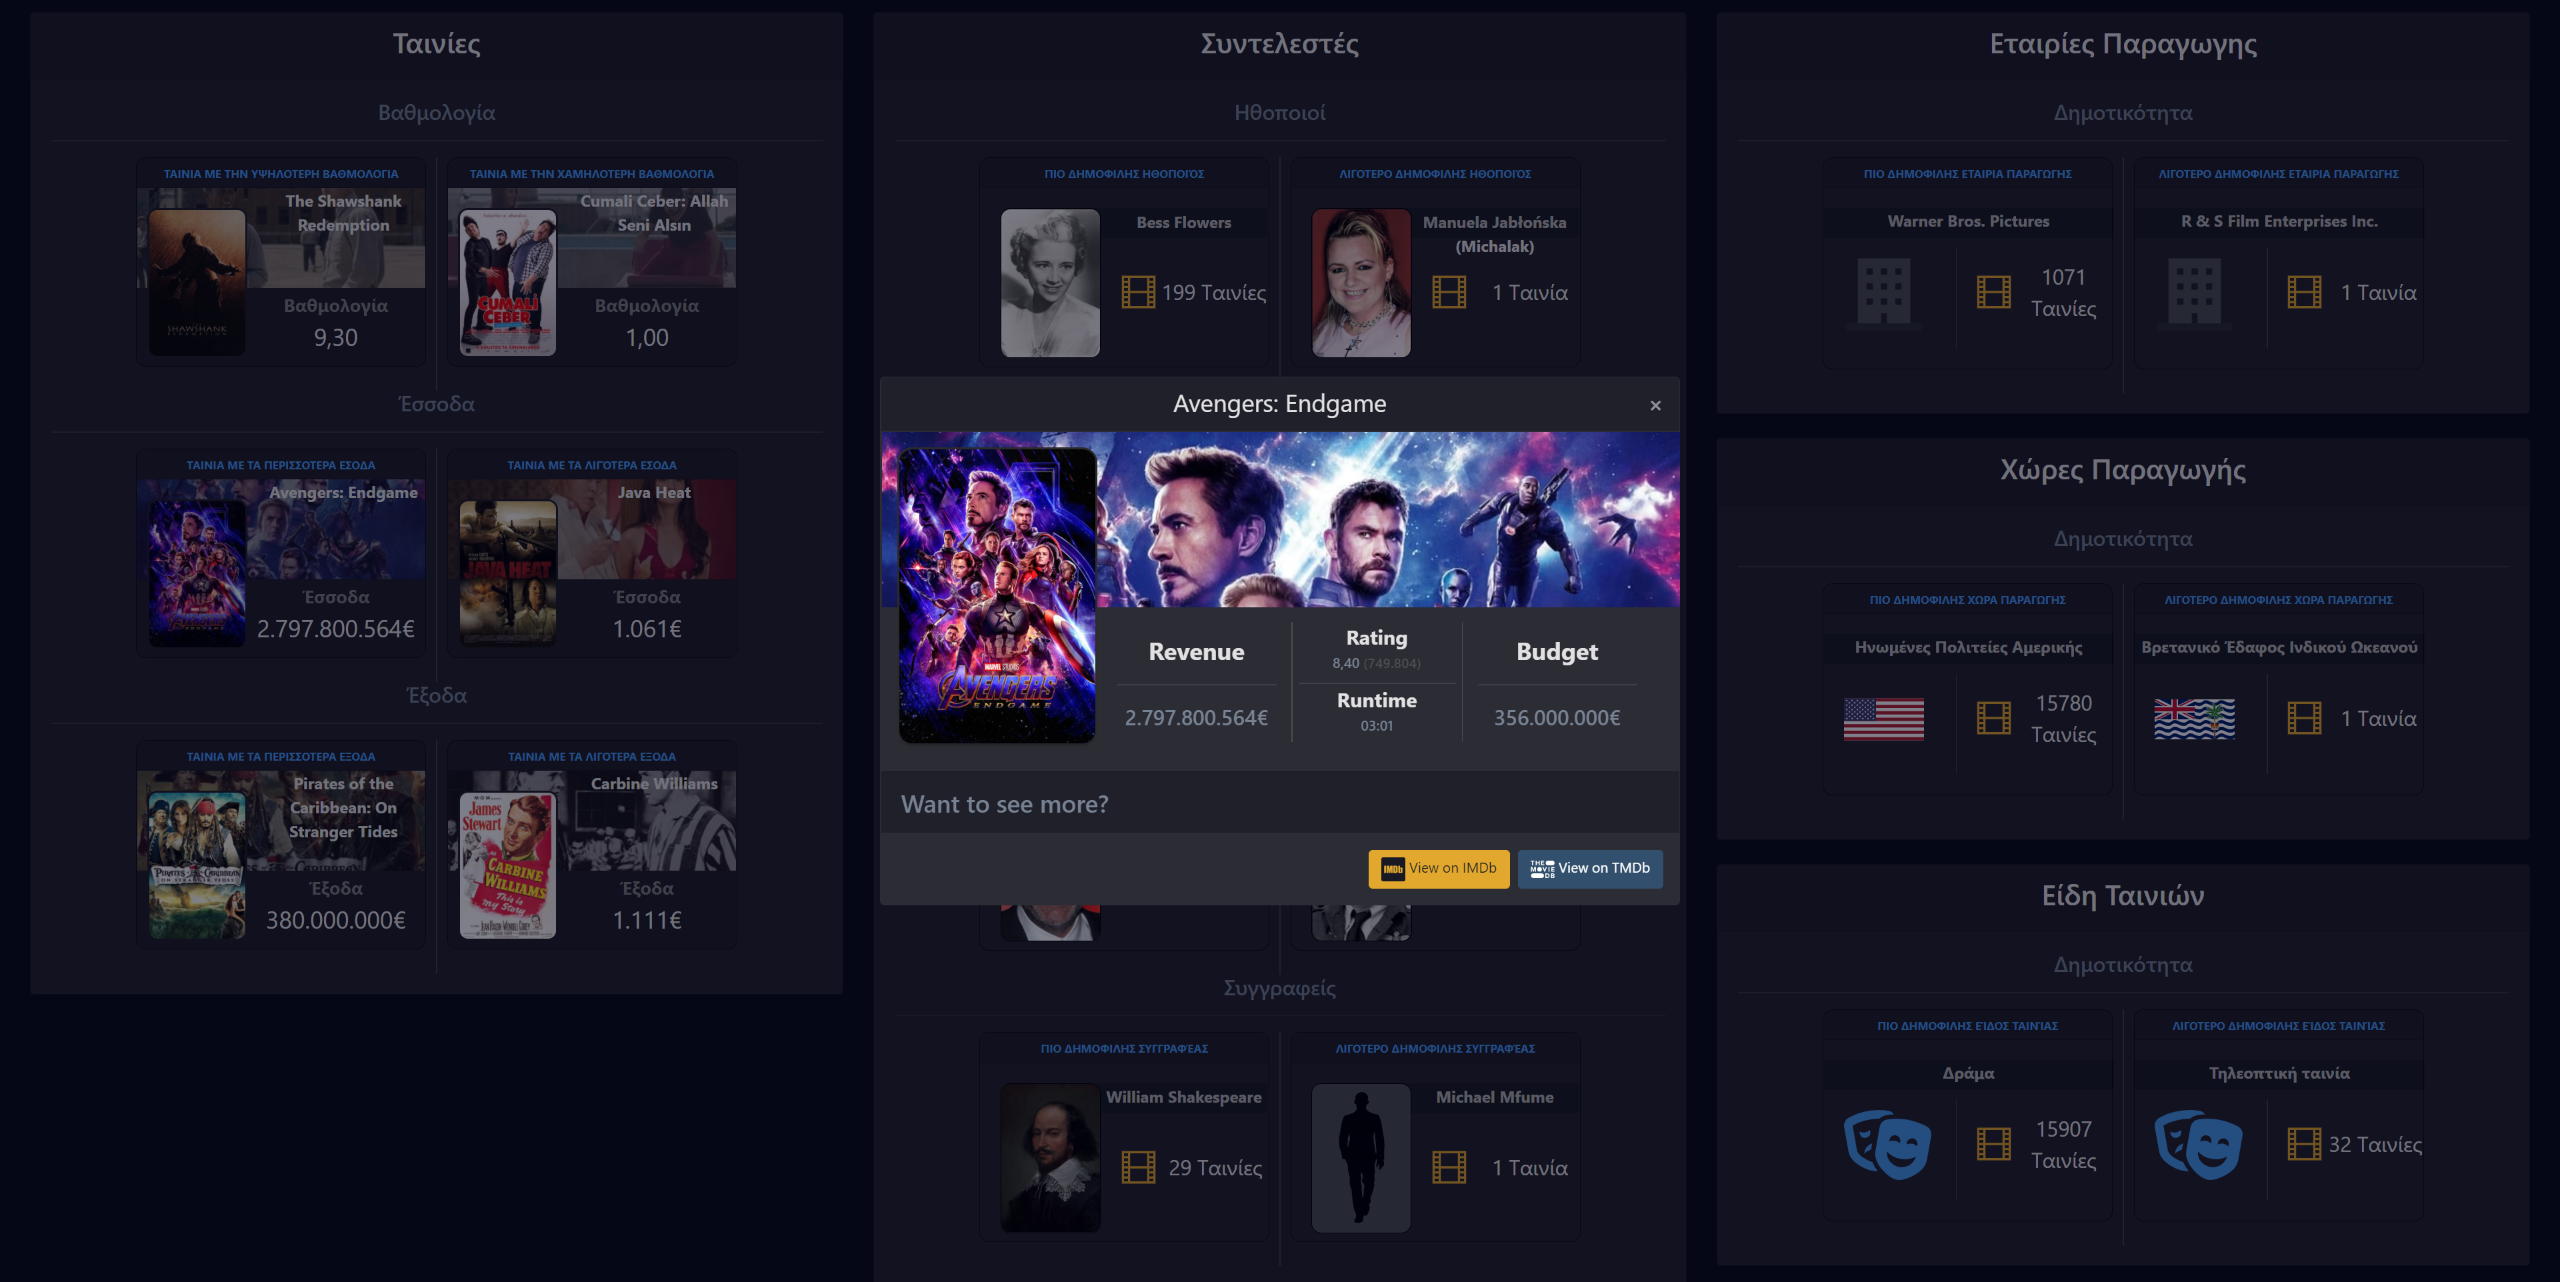
\includegraphics[width=145mm]{Chapters/6 - Manual/Images/main_page_insights_modal.png}
  \caption{Παράθυρο προβολής στοιχείων ταινίας}
  \label{demo:movie:modal}
\end{figure}

Στις υπόλοιπες κατηγορίες εμφανίζονται μόνο οι πιο δημοφιλής και λιγότερο δημοφιλής σε σχέση με την συμμετοχή τους σε ταινίες γενικότερα. Όταν ο χρήστης πατήσει σε μια κάρτα στις υπόλοιπες κατηγορίες η γενική κατηγορία της εφαρμογής θα αλλάξει και θα εμφανίσει στοιχεία της επιλογής του χρήστη.


